\section{Results}\label{section:eval-results}

% Commands to edit stats which might change later. 

% demographic questions
\newcommand{\participantsCount}{20}
\newcommand{\participantsMale}{17}
\newcommand{\participantsAge}{26}

% model viewer statistical facts
\newcommand{\evalExpMvAvgPoses}{3.255} %TODO: correct value
\newcommand{\evalExpMvStdPoses}{2.284}
\newcommand{\evalExpMvParticipants}{12}

% avg lp experiments
\newcommand{\kammAvgHits}{36.23/60}
\newcommand{\kammAvgStd}{6.87/60}
\newcommand{\pietAvgHits}{2.60}
\newcommand{\pietAvgStd}{0.734}
% TODO: adjust values
\newcommand{\oursAvgHits}{32/30}
\newcommand{\oursAvgStd}{2/30}

% model viewer sus scores
\newcommand{\evalExpMvSusScore}{82}
\newcommand{\evalExpMvSusGrade}{B}
\newcommand{\evalExpMvSusAdj}{\enquote{Good}}

% model viewer sus scores
\newcommand{\evalExpLpSusScore}{82}
\newcommand{\evalExpLpSusGrade}{B}
\newcommand{\evalExpLpSusAdj}{\enquote{Good}}

% model viewer sus scores
\newcommand{\evalExpVkSusScore}{82}
\newcommand{\evalExpVkSusGrade}{B}
\newcommand{\evalExpVkSusAdj}{\enquote{Good}}


% Calculations
\newcommand{\participantsFemale}{\pgfmathparse{\participantsCount - \participantsMale}\pgfmathprintnumber[fixed, precision=4]{\pgfmathresult}}%chktex 8 chktex 1

% First try in performing a T-Test. TODO: Check with michael
% \pgfmathparse{10/6.5}\pgfmathprintnumber[fixed, precision=4]{\pgfmathresult}

% This evaluation of the preliminary questions is pretty WIP.

\participantsCount{} persons participated in the evaluation. \participantsFemale{} stated, they identify as female and \participantsMale{} identify as male. The average was \participantsAge{} years. 
% TODO: table of main disciplines and degrees
The main disciplines and degrees are shown in Table TODO.
% TODO: show graph of A5 questions
All users (100\%) use their smartphone multiple times a day, as seen in Figure TODO. Most participants  (TODO: PERCENTAGE) use their computer for work or studies TODO. They (TODO: PERCENTAGE) play computer games TODO.  A huge portion (TODO: PERCENTAGE) use \ac{VR} less than one time a month.
%The evaluation was conducted during different times of the day. does say nothing


\subsection{Model Viewer}\label{section:eval-res-mv}

The model viewer experiment, described in Section~\ref{subsection:model-viewer}, allows users to view a \ac{3D} model from different angles. To benchmark extensive usage, a second model instance in another color (the target) is spawned after starting the task. Since in the current implementation, the model cannot be rotated upside down (as mentioned in Section~\ref{subsection:topic-data}), the target is spawned with random reachable orientations.
As soon as the task is started, the user has 30 seconds to match as many orientations as possible. Similar to the implementation by \citeauthor{Katzakis.2010}, the target is rotated to a new random orientation, after one orientation was matched~\cite[140]{Katzakis.2010}.
Because it is hard to match the rotation exactly on all three axes, it is enough to pose the model in a similar orientation to the target. A similar pose is reached, when the smallest angle between the two rotations is less than 20 radians.

\begin{figure}[H]
  \centering
  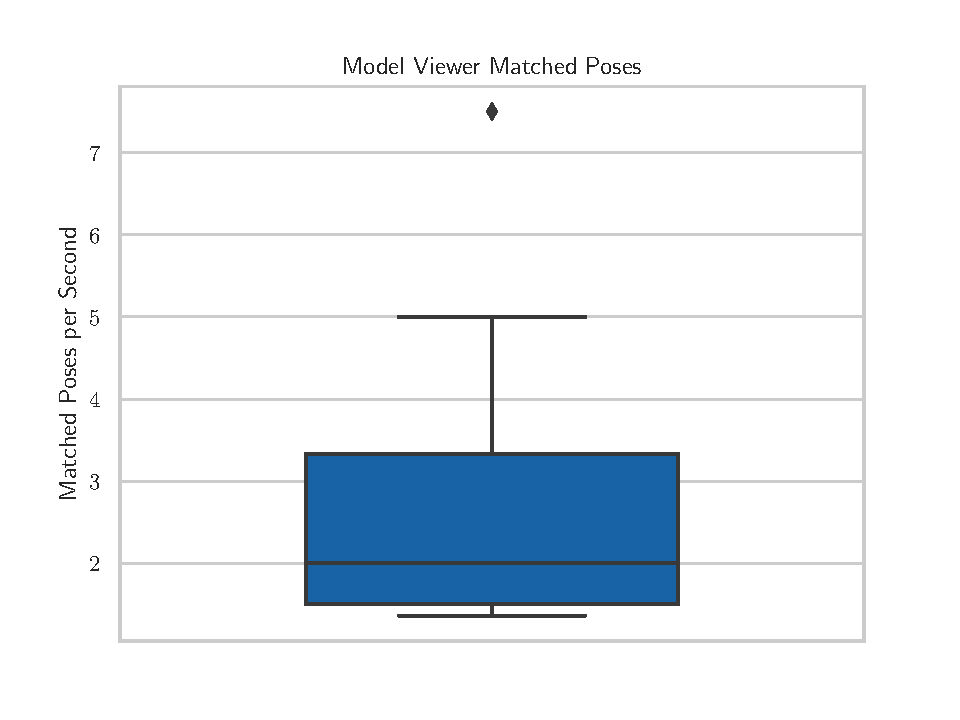
\includegraphics[width=10cm]{figures/evaluation/eval_exp_mv.pdf}
  \caption[Model viewer experiment results]{The time in seconds it took to match a correct pose in the model viewer experiment.}\label{fig:eval-exp-mv}
\end{figure}

% TODO: T-Test:
%\pgfmathparse{(\evalExpMvAvgPoses-6.5)/(\evalExpMvStdPoses/sqrt(\evalExpMvParticipants))}\pgfmathprintnumber[fixed, precision=4]{\pgfmathresult} 
% chktex 1
As seen in Figure~\ref{fig:eval-exp-mv}, the average time it took to match a correct poses is roughly \evalExpMvAvgPoses{} seconds. \citeauthor{Katzakis.2010} tracked the time it takes to match a pre-defined pose with a Smartphone, a mouse and a touch panel. The lowest time in average to match one pose, 6.5 seconds, was achieved using the Smartphone as input device~\cite[140]{Katzakis.2010}. The average time to match a pose of the model viewer (\evalExpMvAvgPoses{} seconds) experiment presented in Chapter~\ref{section:eval-res-mv} is lower than the average of the evaluation of \citeauthor{Katzakis.2010} (6.5 seconds). This can be due to the fact that users never had to turn the smartphone completely upside down, since rotations were chosen to be always upside up, because of the previously mentioned limitation. Another advantage of the presented implementation is, that the target and the controlled model are not displayed in two separate locations like in {\citetitle{Katzakis.2010}}, but rather with the same origin in the same coordinate space, which makes it easier to see the difference between both rotations~\cite[140]{Katzakis.2010}. Also the fact that a skeleton model instead of a multi-colored cube was used, could play a role. 

\begin{figure}[H]
  \centering
  \begin{subfigure}{.45\textwidth}%
    \centering
    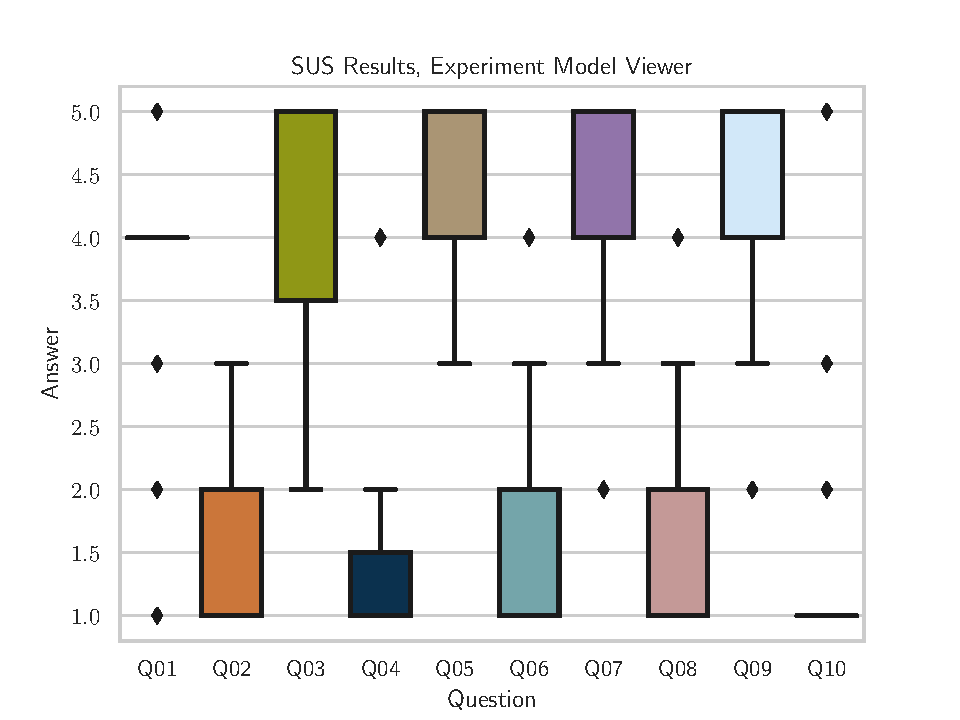
\includegraphics[width=\textwidth]{figures/evaluation/res_exp_mv.pdf}
    \caption{The results of question one to ten.}\label{fig:res-exp-mv}
  \end{subfigure}%
  \hspace{0.1\textwidth}%
  \begin{subfigure}{.45\textwidth}%
    \centering
    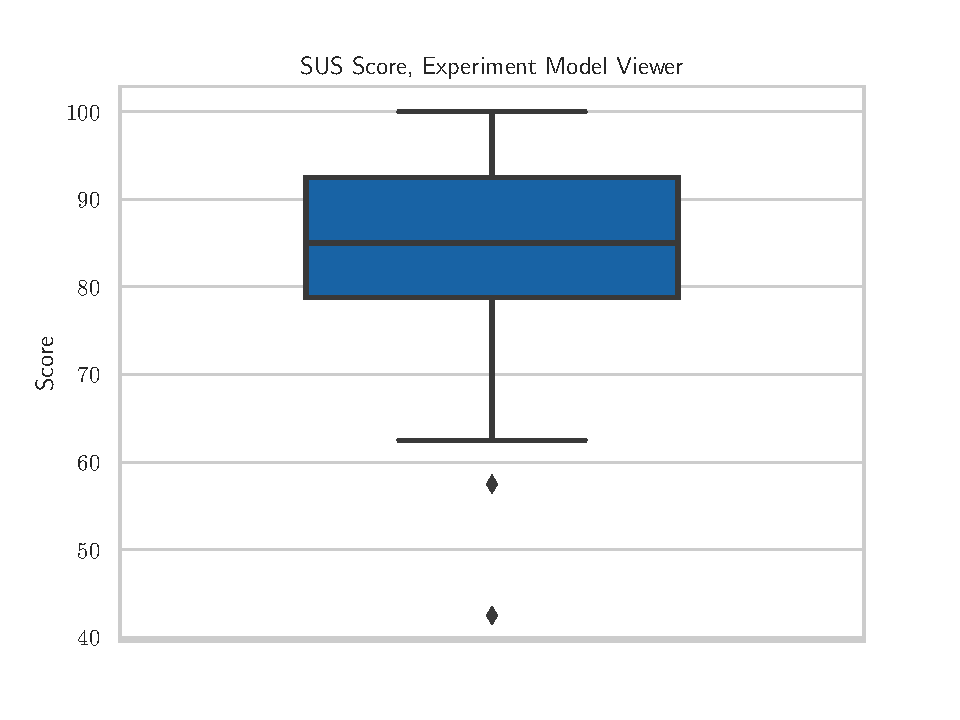
\includegraphics[width=\textwidth]{figures/evaluation/score_exp_mv.pdf}
    \caption{The overall \ac{SUS} score.}\label{fig:score-exp-mv}
  \end{subfigure}%
  \caption[User study results of the model viewer experiment]{The results of the \ac{SUS} user study for the model viewer.}\label{fig:exp-mv-stats}
\end{figure}

However, also the \ac{SUS} study results indicate a useable implementation, as seen in Figure~\ref{fig:exp-mv-stats}. A score of \evalExpMvSusScore\ is considered \evalExpMvSusAdj\ and mapped to the grade \evalExpMvSusGrade, according to \citeauthor{Bangor.2009}~\cite[120\psq]{Bangor.2009}.



\subsection{Laser Pointer}\label{section:eval-res-lp}

Section~\ref{subsection:laser-pointer} introduces the laser pointer experiment. To test the performance of participants using this interaction, three cubes (the targets) are spawned at random locations in front of the user. He has to select as much cubes as possible in 30 seconds. The user was told to be as fast and especially as accurate as possible, since miss-hits are counted. 

To trigger a selection, the user has to touch the smartphone display. This counts as a click. If no cube was selected, a miss is counted. The total selection (click) count is the sum of hits and miss-clicks. If one cube was hit, another one is spawned, so that always three cubes are visible. This is important, because the user can plan to hit the next target while currently aiming for the current one. Otherwise the task would test the users reaction time, which is not desired. 

\begin{figure}[H]
  \centering
  \begin{subfigure}{.45\textwidth}%
    \centering
    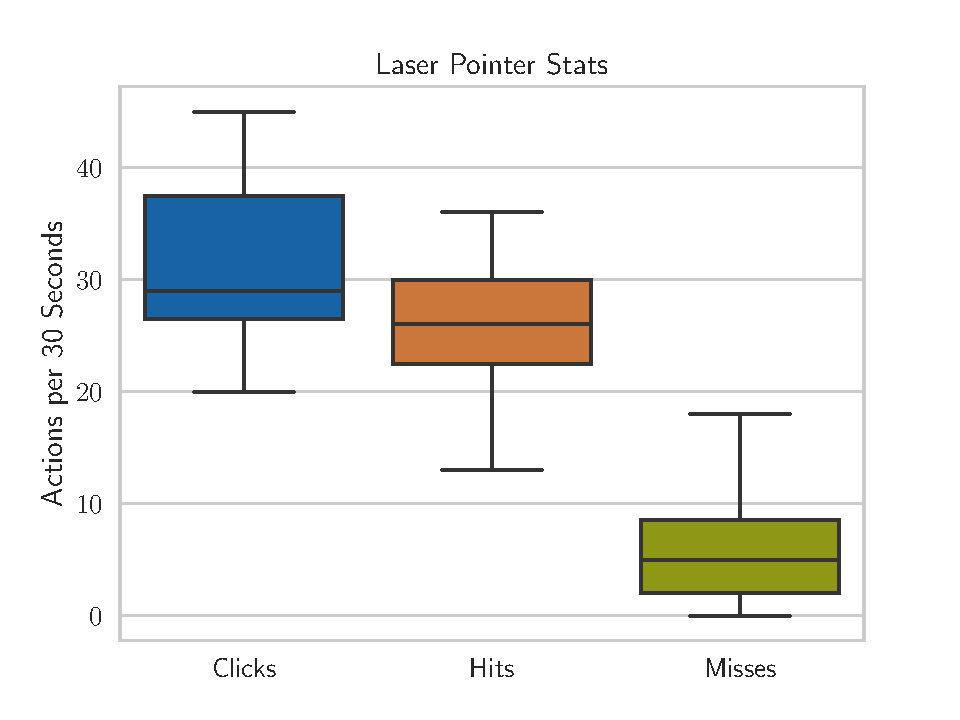
\includegraphics[width=\textwidth]{figures/evaluation/eval_exp_lp.pdf}
    \caption{The count of clicks, hits and misses per 30 seconds. Clicks are the sum of hits and misses.}\label{fig:eval-exp-lp}
  \end{subfigure}%
  \hspace{0.1\textwidth}%
  \begin{subfigure}{.45\textwidth}%
    \centering
    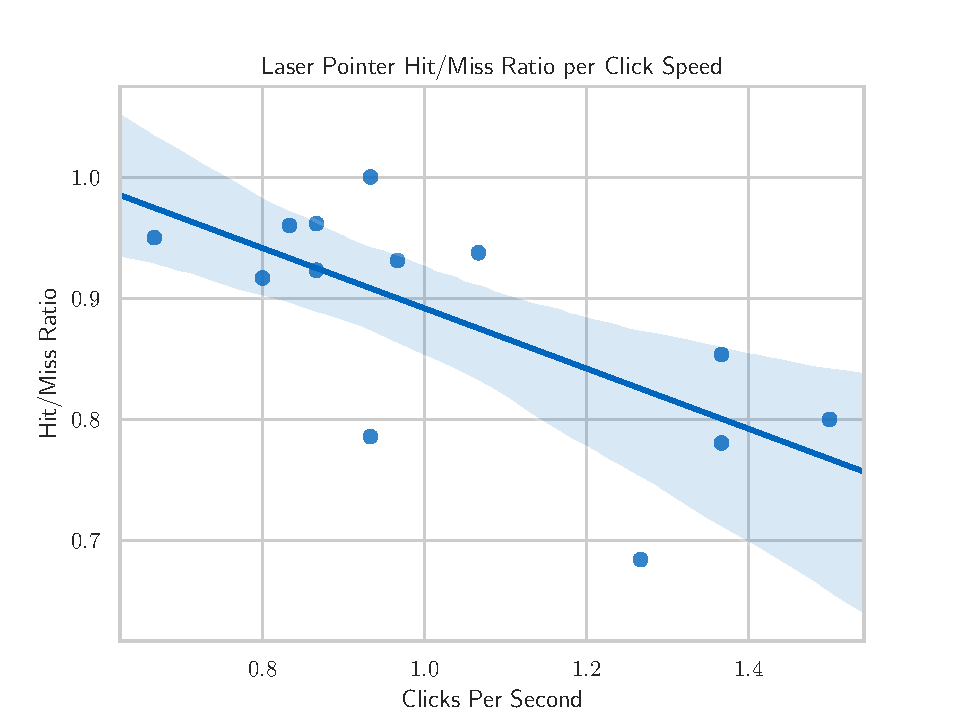
\includegraphics[width=\textwidth]{figures/evaluation/eval_exp_lp_ratio_scatter.pdf}
    \caption{The Hit/Miss ratio per click speed. The line visualizes the linear regression with a 95\% confidence interval.}\label{fig:eval-exp-lp-ratio-scatter}
  \end{subfigure}%
  \caption[Laser pointer experiment results]{The results of the laser pointer experiment.}\label{fig:exp-lp-eval}
\end{figure}

% TODO as seen in fig~\ref{fig:eval-exp-lp} is roughly...

Figure~\ref{fig:eval-exp-lp-ratio-scatter} % TODO: shows the hit mis ratio per click speed


The performance of this experiment is hard to compare with other implementations, without a standardized experiment setup. For example the size, shape, position and distance of the targets but also the spawn area and wether distracting elements are present or not, varies between different task evaluations of other research. However a comparison should still give a rough estimate wether the performance is similar, much better or really bad. Often the hit count is measured in different time intervals. To compare the results, the average hit count per second is calculated.

\citeauthor{Kamm.2018} tested his implementation in a similar \ac{VR} scenario with a wrist band as input device. To compare his implementation, he also tested a laser pointer approach using a \ac{VR} motion controller~\cite[39]{Kamm.2018}. A major difference to his experiment setup is, that only one target is displayed at a time. Another difference is, that the user has to rotate his head more in order to see the targets, since they are placed in a 90 degrees radius. An arrow, which always points to the next target, is displayed to prevent wasting time while searching for the next one. Also the distance from the user to the targets is randomized~\cite[45]{Kamm.2018}.

\citeauthor{Pietroszek.2014} compared a smartphone and a Wii Remote as interaction device for a large display. The task was to move the pointer from one point to another~\cite[124]{Pietroszek.2014}. To compare it with the presented experiments, the results of the one without distraction elements using the smartphone is used. 

\begin{table}
  \centering
    \begin{tabular}{l c c}
    \toprule
    Research & Average Hits per Second & Standard Derivation\\
    \midrule
    \cite{Kamm.2018} & \pgfmathparse{\kammAvgHits}\pgfmathprintnumber[fixed, precision=3]{\pgfmathresult} & \pgfmathparse{\kammAvgStd}\pgfmathprintnumber[fixed, precision=3]{\pgfmathresult}\\%chktex 2 
    \cite{Pietroszek.2014} & \pietAvgHits{} & \pietAvgStd{} \\%2.60s,  = .734) %chktex 2 21
    Chapter~\ref{section:eval-res-lp} & \pgfmathparse{\oursAvgHits}\pgfmathprintnumber[fixed, precision=3]{\pgfmathresult} & \pgfmathparse{\oursAvgStd}\pgfmathprintnumber[fixed, precision=3]{\pgfmathresult}\\
    \bottomrule
    \end{tabular}
  \caption[Comparison of laser pointer task results from other research.]{Comparison of the average hits per second from similar laser pointer experiments of other research.}\label{tab:lp-comp}
\end{table}

% TODO: explain tab~\ref{tab:lp-comp} and conclude


\begin{figure}[H]
  \centering
  \begin{subfigure}{.45\textwidth}%
    \centering
    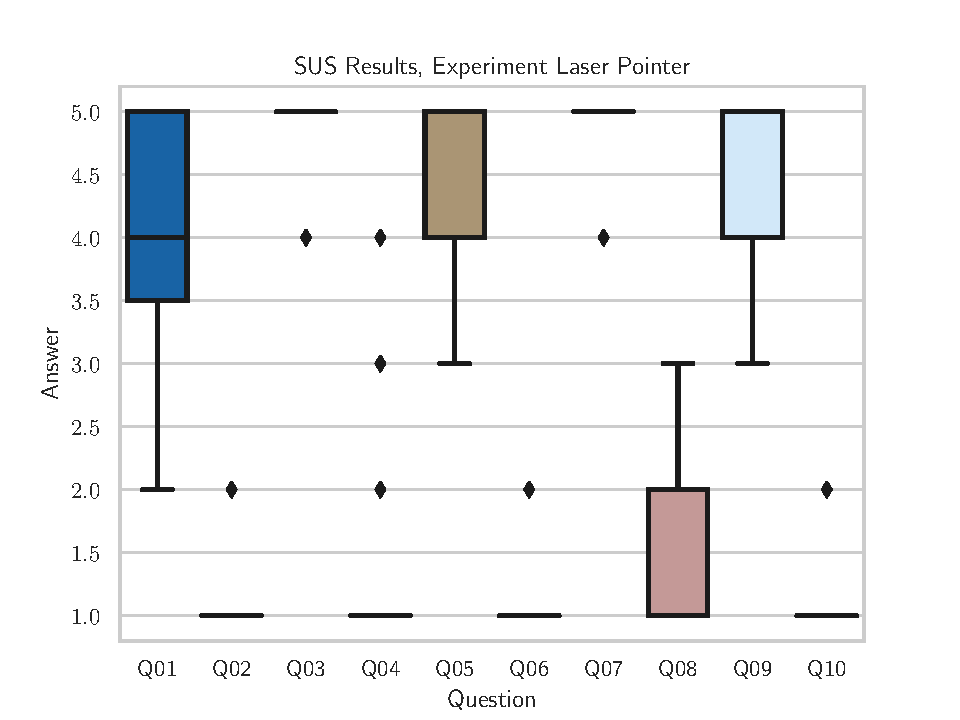
\includegraphics[width=\textwidth]{figures/evaluation/res_exp_lp.pdf}
    \caption{The results of question one to ten presented as box plots.}\label{fig:res-exp-lp}
  \end{subfigure}%
  \hspace{0.1\textwidth}%
  \begin{subfigure}{.45\textwidth}%
    \centering
    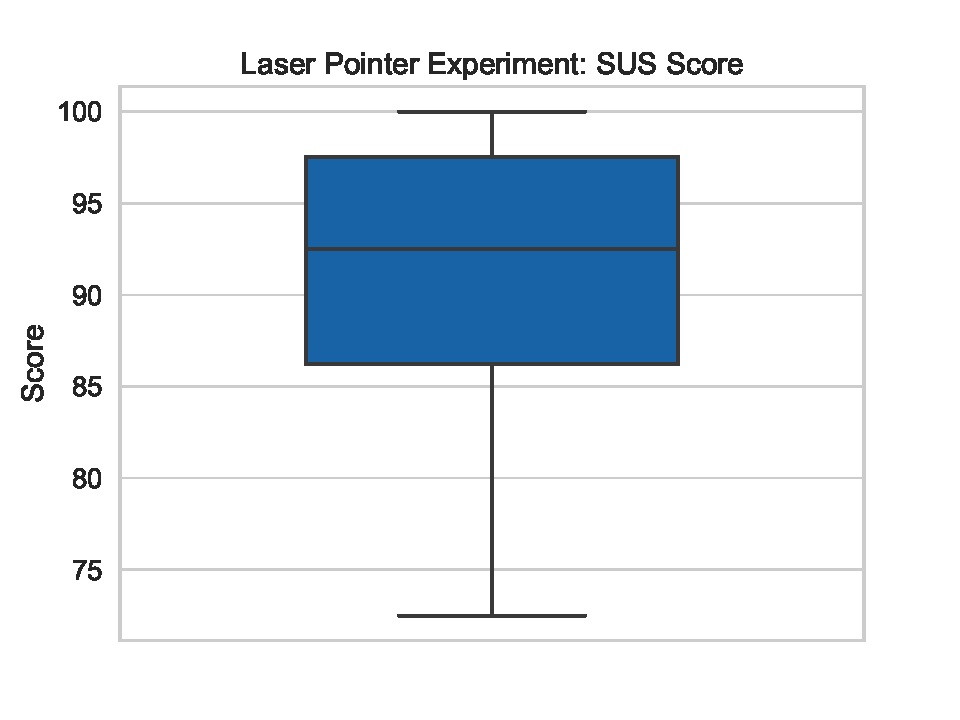
\includegraphics[width=\textwidth]{figures/evaluation/score_exp_lp.pdf}
    \caption{The overall \ac{SUS} score presented in a box plot.}\label{fig:score-exp-lp}
  \end{subfigure}%
  \caption[User study results of the laser pointer experiment]{The results of the \ac{SUS} user study for the laser pointer.}\label{fig:exp-lp-stats}
\end{figure}

However, not only the measured interaction times but also the \ac{SUS} study results indicate a useable implementation, as seen in Figure~\ref{fig:exp-lp-stats}. A score of \evalExpLpSusScore\ is considered \evalExpLpSusAdj\ and mapped to the grade \evalExpLpSusGrade, according to \citeauthor{Bangor.2009}~\cite{Bangor.2009}.



\subsection{Virtual Keyboard}\label{section:eval-res-vk}


% TODO. VK still has to be evaluated
\begin{figure}[H]
  \centering
  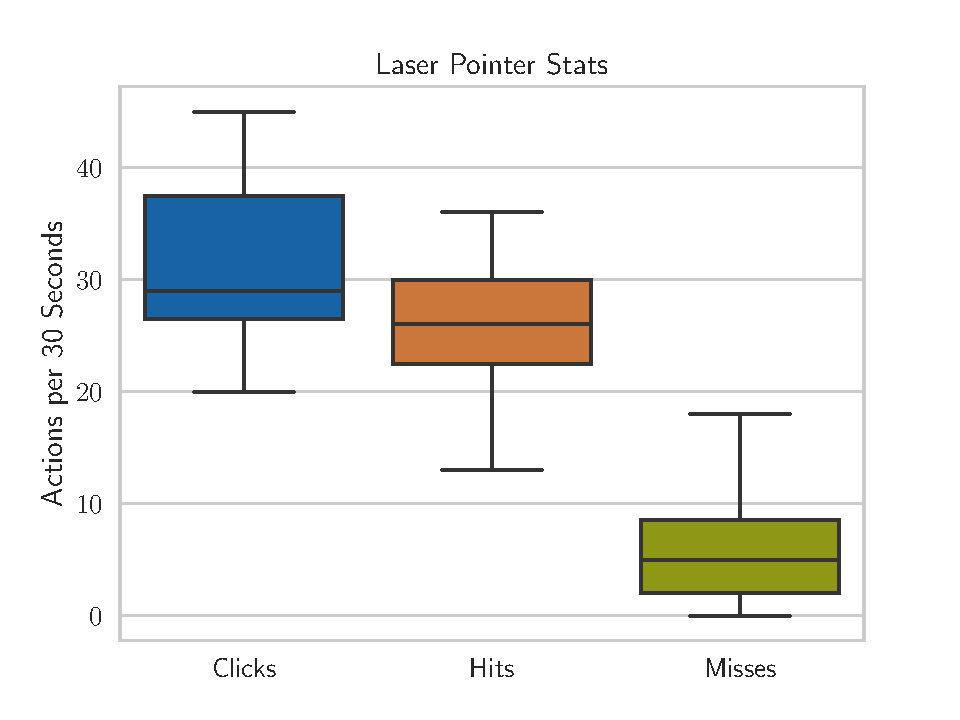
\includegraphics[width=10cm]{figures/evaluation/eval_exp_lp.pdf}
  \caption[TO DO]{TO DO}\label{fig:eval-exp-vk}
\end{figure}


\begin{figure}[H]
  \centering
  \begin{subfigure}{.45\textwidth}%
    \centering
    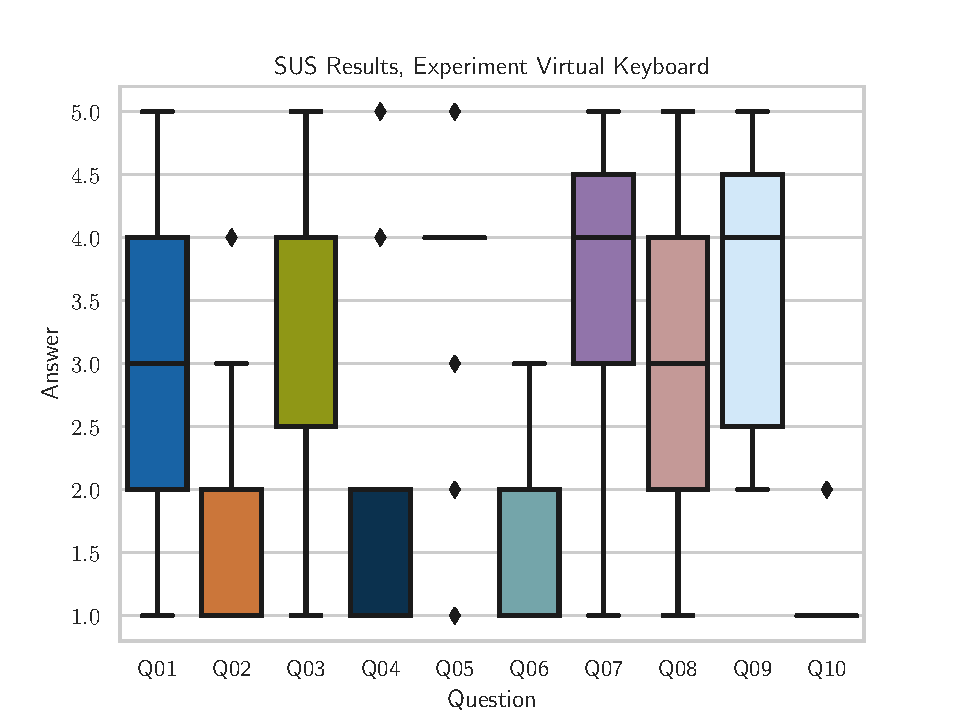
\includegraphics[width=\textwidth]{figures/evaluation/res_exp_vk.pdf}
    \caption{The results of question one to ten.}\label{fig:res-exp-vk}
  \end{subfigure}%
  \hspace{0.1\textwidth}%
  \begin{subfigure}{.45\textwidth}%
    \centering
    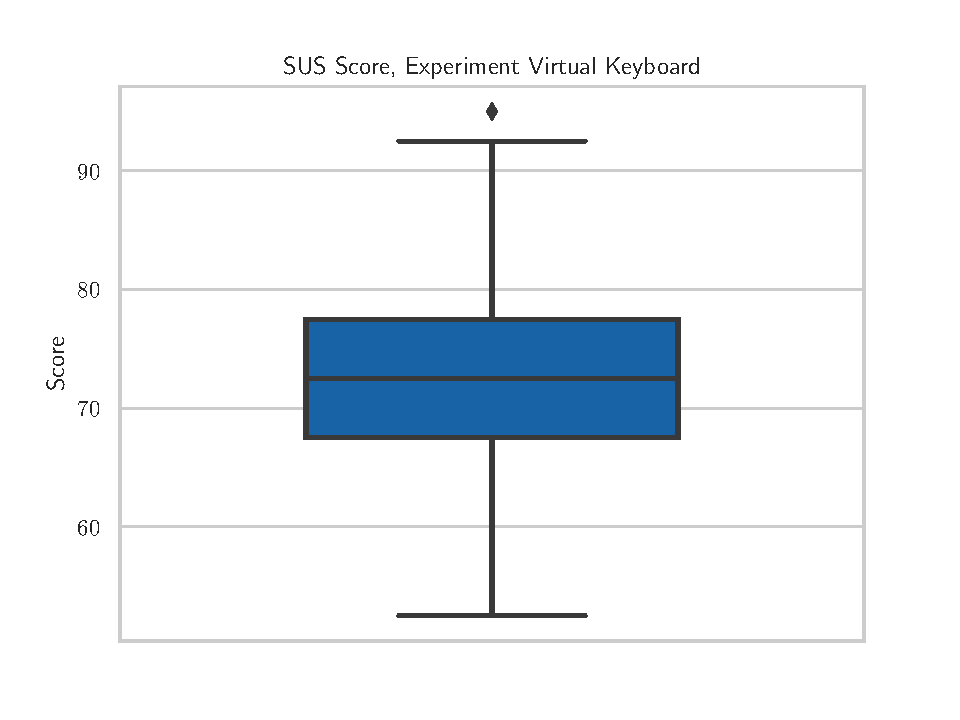
\includegraphics[width=\textwidth]{figures/evaluation/score_exp_vk.pdf}
    \caption{The overall \ac{SUS} score.}\label{fig:score-exp-vk}
  \end{subfigure}%
  \caption[User study results of the virtual keyboard experiment]{The results of the \ac{SUS} user study for the virtual keyboard.}\label{fig:exp-vk-stats}
\end{figure}

However, not only the measured interaction times but also the \ac{SUS} study results indicate a useable implementation, as seen in Figure~\ref{fig:exp-mv-stats}. A score of \evalExpVkSusScore\ is considered \evalExpVkSusAdj\ and mapped to the grade \evalExpVkSusGrade, according to \citeauthor{Bangor.2009}~\cite{Bangor.2009}.